\section{How are we going to get there}

\subsection{Leading by example}

The principal technique throughout this book is leading by
example. What this means in this case is that the ideas are presented
primarily in terms of a coherent collection of examples, rendered as
\texttt{Scala} code, that work together to do something. Namely, these
examples function together to provide a prototypical web-based
application with a feature set that resonates with what application
developers are building today and contemplating building tomorrow.

Let's illustrate this in more detail by telling a story. We imagine a
cloud-based editor for a simple programming language, not unlike
\texttt{Mozilla}'s \texttt{bespin} . A user can register with the
service and then create an application project which allows them
\begin{itemize}
   \item to write code in a structured editor that understands the language;
   \item manage files in the application project;
   \item compile the application;
   \item run the application
\end{itemize}

\begin{figure}[tbp]
\begin{center}
{ \includegraphics[scale=.35]{/Users/lgm/work/src/projex/biosimilarity/trace/src/main/book/content/figures/RLambdaSignupPageScreenShot.pdf} }
\caption{ Example sign up page }
\end{center}
\end{figure}

% Thus, at broad strokes requests from the client app to the server break down into the following categories
% \begin{itemize}
%   \item edits to code
%   \item edits to project structure
%   \item compilation and execution requests
% \end{itemize}

These core capabilities wrap around our little toy programming
language in much the same way a modern IDE might wrap around
development in a more robust, full-featured language. Hence, we want
the capabilities of the application to be partially driven from the
specification of our toy language. For example, if we support some
syntax-highlighting, or syntax-validation on the client, we want that
to be driven from that language spec to the extent that changes to the
language spec ought to result in changes to the behavior of the
highlighting and validation. Thus, at the center of our application is
the specification of our toy language.

\begin{figure}[tbp]
\begin{center}
{ \includegraphics[scale=.35]{/Users/lgm/work/src/projex/biosimilarity/trace/src/main/book/content/figures/RLambdaREPLPageScreenShot.pdf} }
\caption{ Example REPL page }
\end{center}
\end{figure}

\begin{figure}[tbp]
\begin{center}
{ \includegraphics[scale=.35]{/Users/lgm/work/src/projex/biosimilarity/trace/src/main/book/content/figures/RLambdaSampleEvaluationResultPage.pdf} }
\caption{ Example evaluation result page }
\end{center}
\end{figure}

\subsubsection{Our toy language}

\paragraph{Abstract syntax}
%For our example we'll need a toy language.
Fittingly for a book about \texttt{Scala} we'll use the
$\lambda$-calculus as our toy language. \footnote{A word to the wise:
  even if you are an old hand at programming language semantics, even
  if you know the $\lambda$-calculus like the back of your hand, you
  are likely to be surprised by some of the things you see in the next
  few sections. Just to make sure that everyone gets a chance to look
  at the formalism as if it were brand new, a few recent theoretical
  developments have been thrown in. So, watch out!} The core
\textit{abstract} syntax of the lambda calculus is given by the
following \textit{EBNF} grammar.

\begin{mathpar}
  \inferrule* [lab=expression] {} {{M,N} ::=}
  \and
  \inferrule* [lab=mention] {} {x}
  \and
  \inferrule* [lab=abstraction] {} {\;| \; \lambda x . M}
  \and
  \inferrule* [lab=application] {} {\;| \; M N}
\end{mathpar} 

Informally, this is really a language of pure variable management. For
example, if the expression $M$ mentions $x$, then $\lambda x. M$ turns
$x$ into a variable in $M$ and provides a means to substitute values
into $M$, via application. Thus, $(\lambda x.M)N$ will result in a new
term, sometimes written $M[N/x]$, in which every occurrence of $x$ has
been replaced by an occurrence of $N$. Thus, $(\lambda x.x)M$ yields
$M$, illustrating the implementation in the $\lambda$-calculus of the
identity function. It turns out to be quite remarkable what you can do
with pure variable management.

\paragraph{Concrete syntax}
We'll wrap this up in concrete syntax.

\begin{mathpar}
  \inferrule* [lab=expression] {} {{M,N} ::=}
  \and
  \inferrule* [lab=mention] {} {x}
  \and
  \inferrule* [lab=abstraction] {} {\;| \; \texttt{(} x_1 \texttt{,} ... \texttt{,} x_k \texttt{)} \; \texttt{=>} \; M}
  \and
  \inferrule* [lab=application] {} {\;| \; M\texttt{(} N_1 \texttt{,} ... \texttt{,} N_k \texttt{)}}
  \and
  \inferrule* [lab=let] {} {\;| \; \texttt{val} \; x \; \texttt{=} \; M \texttt{;} N}
  \and
  \inferrule* [lab=seq] {} {\;| \; M \texttt{;} N }
  \and
  \inferrule* [lab=group] {} {\;| \; \texttt{ \{ } M \texttt{ \} } }
\end{mathpar} 

It doesn't take much squinting to see that this looks a lot like a
subset of \texttt{Scala}, and that's because -- of course! --
functional languages like \texttt{Scala} all share a common core that
is essentially the $\lambda$-calculus. Once you familiarize yourself
with the $\lambda$-calculus as a kind of design pattern you'll see it
poking out everywhere: in \texttt{Clojure} and \texttt{OCaml} and
\texttt{F\#} and \texttt{Scala}. In fact, as we'll see later, just
about any DSL you design that needs a notion of variables could do
worse than simply to crib from this existing and well understood
design pattern.

\begin{figure}[tbp]
\begin{center}
{ 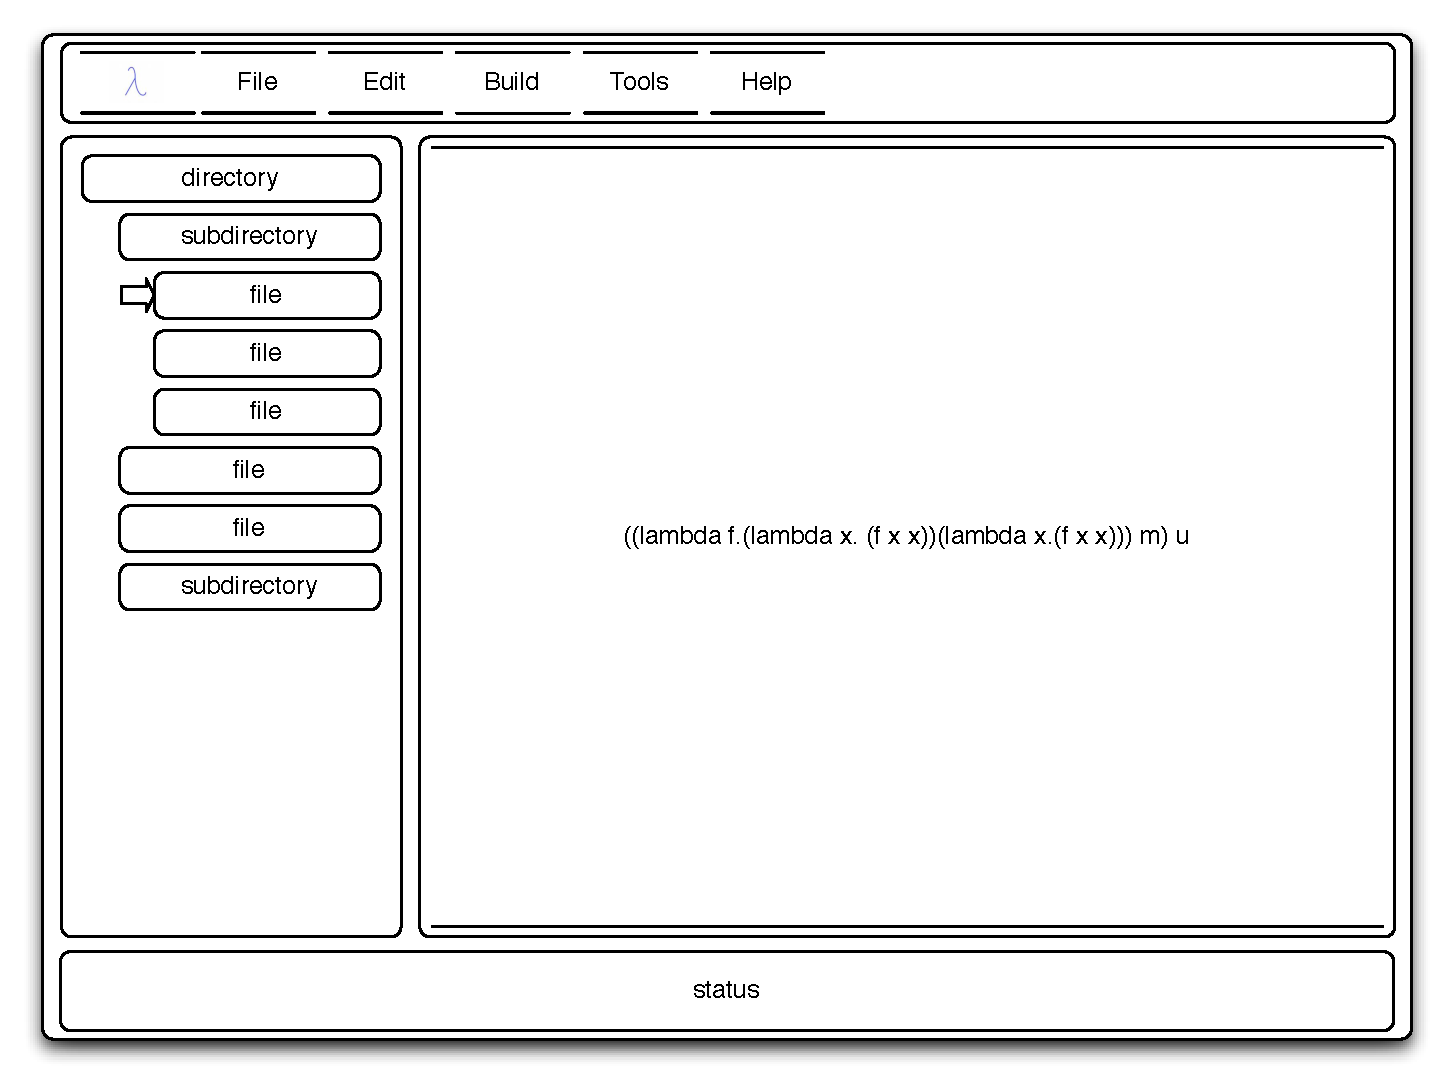
\includegraphics[scale=.65]{/Users/lgm/work/src/projex/biosimilarity/trace/src/main/book/content/figures/ProjectEditor.pdf} }
\caption{ Project and code editor }
\end{center}
\end{figure}

\subsubsection{Code editor}

\subsubsection{Project editor}

\subsubsection{Advanced features}

\subsection{Chapter map}

Taking a step back from the technical discussion let's recall what we
plan to cover and how we plan to cover it. Essentially, the book is
organized to follow the processing of \texttt{HTTP} requests from the
browser through the server and application code out to the store and
back.

\begin{itemize}
\item Chapter two introduces terminology, notation and concepts
  necessary for the rest of the book.
\item Chapter three looks at the organization of an \texttt{HTTP} server.
\item Chapter four investigates parsing the transport and application
  level requests.
\item Chapter five focuses on the application domain model.
\item Chapter six addresses at the navigation model.
\item Chapter seven reviews collections.
\item Chapter eight looks at the storage model.
\item Chapter nine investigates deployment of the application.
\item Chapter ten addresses new foundations for semantic query.
\end{itemize}

\begin{figure}[tbp]
\begin{center}
{ 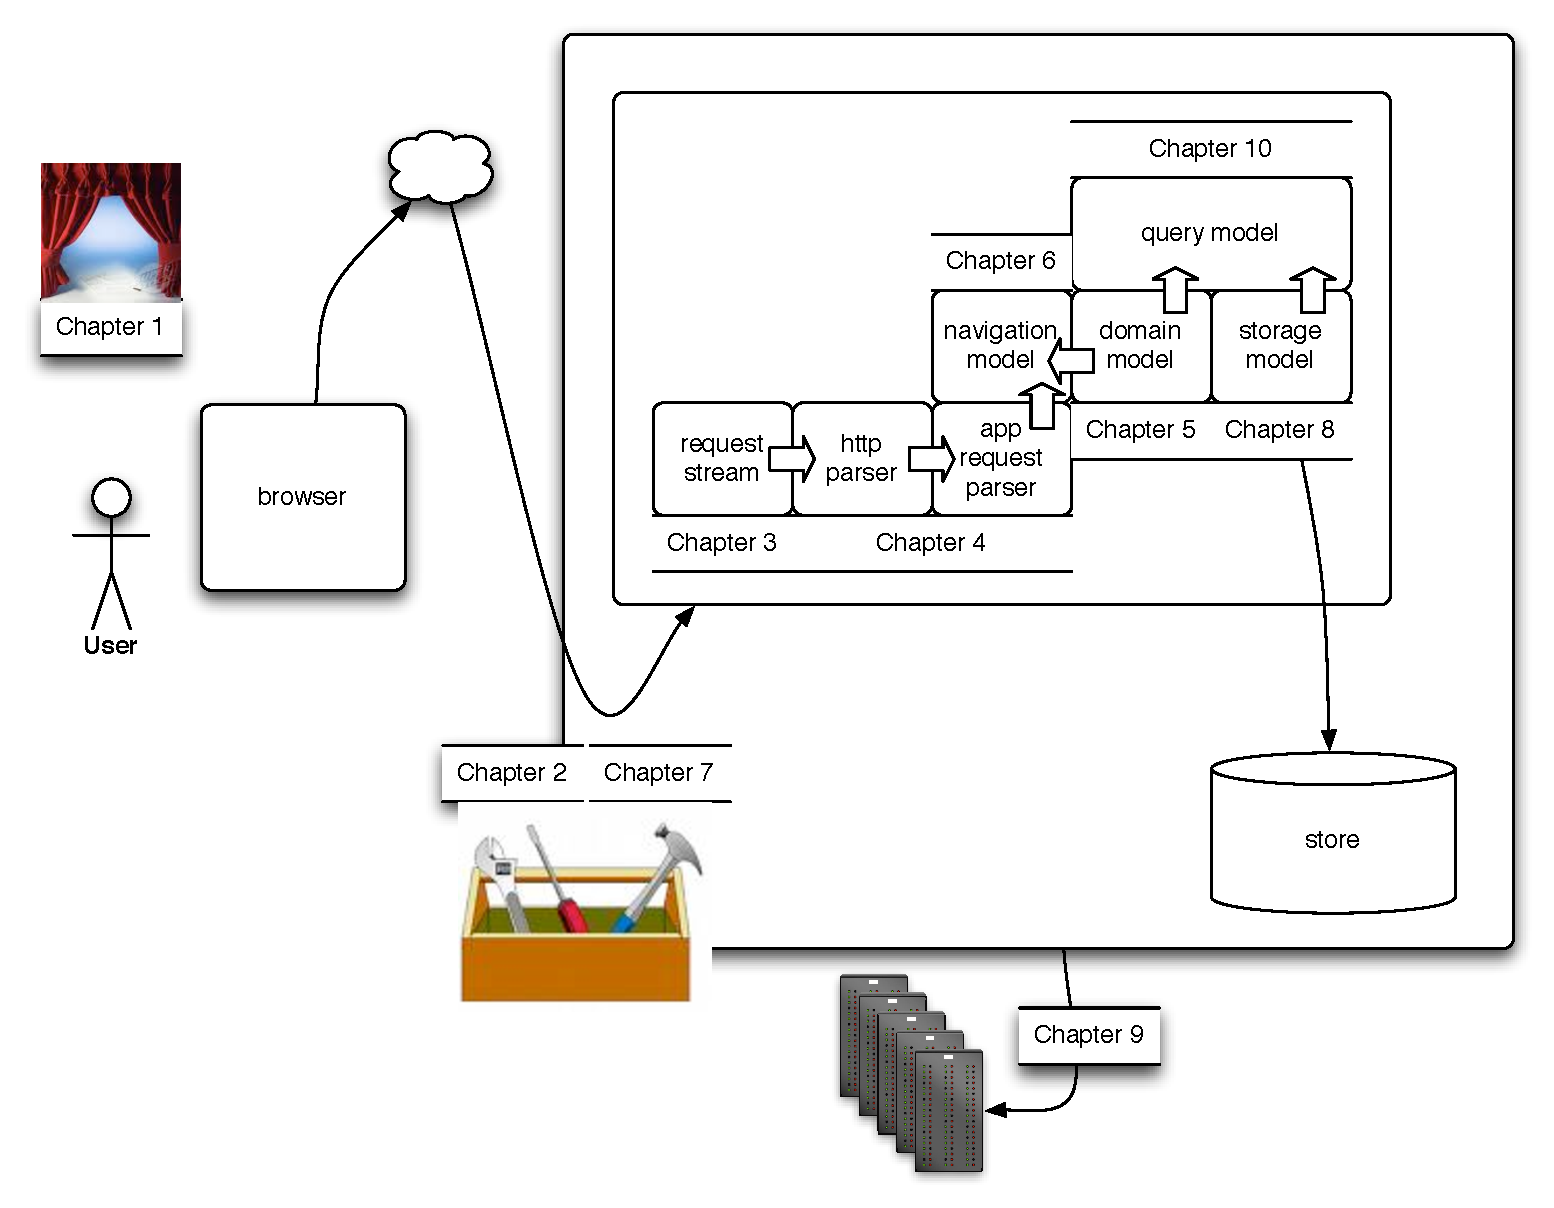
\includegraphics[scale=.65]{/Users/lgm/work/src/projex/biosimilarity/trace/src/main/book/content/figures/MonadicDesignPatternsChapterMap2.pdf} }
\caption{ Chapter map }
\end{center}
\end{figure}